\section{Numerical Computation by Simulation}
\label{sec:numerical}

It may be possible that one wishes to compute distributions, on
irregular regions, for which there is no closed form solution.
Numerically it is straight-forward to calculate the function
$g(t)$. There are two obvious approaches:
\begin{itemize}

\item Numerical computation of a $n$-dimensional integral over
  $\Omega$, or

\item Simulation of the problem, and estimation of the density from
  simulated results. 

\end{itemize}
The two approaches have different advantages and disadvantages. The
former approach has no stochastic component, and so errors are
predictable and regular. 

The later approach allows complex, potentially non-convex,
non-uniform, problems to be solved as long as they can be
simulated. Given the stochastic nature of the latter, it may help to
say a little more:

The general process is as follows:
\begin{enumerate}

\item Simulate a set of $2N$ points in the region of interest, and
  calculate the distances between successive pairs. The region may be
  irregular, or even non-convex; decisions may be made about some
  lines being inadmissable (because, for instance, they are exterior
  to the region for a non-convex region), or distances may be
  non-Euclidean, or the point distribution can be non-uniform. All
  that is needed is a set of output distances $\{ t_i \}_{i=1}^{N}$.

\item The density could then be approximate through binning, or a
  kernal smoothing technique, but in fact, we don't need direct access
  to the density as the estimator uses the Laplace transform.

\end{enumerate}

We have tested the above approach, running it 30 times (with different
seeds), in Matlab for various values of $N$. The results are shown in
Figure~\ref{fig:simulated_laplace}. The first plot shows estimates of
the mean relative absolute error of the estimated Laplace transforms
over the range $S \in [0, 50]$. We can see from the fitted straight
line, that the errors decrease as $1/\sqrt{N}$, dropping to around 1\%
at around $N=100,000$.


....





The second plot shows the computation times\footnote{Both algorithms
  were implemented in Matlab, the exact method using Matlab's {\tt
    quadqk} function. } relative to the computation times for the
``exact'' method\footnote{Note that both techniques are in some
  respect numerical, because even when we have a closed form solution
  for the density, we still typically need to numerically integrate
  this to obtain the Laplace transform, but we shall refer to this
  solution as ``exact'' for the sake of clarity in the following
  results, and because in the following we perform numerical
  integration with error tolerances of $10^{-6}$, which means the
  errors in this approach are significantly smaller than those of the
  simulation-based approach, at least for the ranges of $N$ tested
  here.}  We can immediately notice that computation times are roughly
linear in $N$, as one might expect. that around the range $N=100,000$,
the simulation approach is competitive with the exact approach.

The simulation-based approach is not as accurate as the exact
numerical approach, however, it accuracy should be sufficient for most
estimation problems, without increasing the computational workload
unduly.
make




\begin{figure}[tbp]
  \begin{center}
        \subfloat[line]{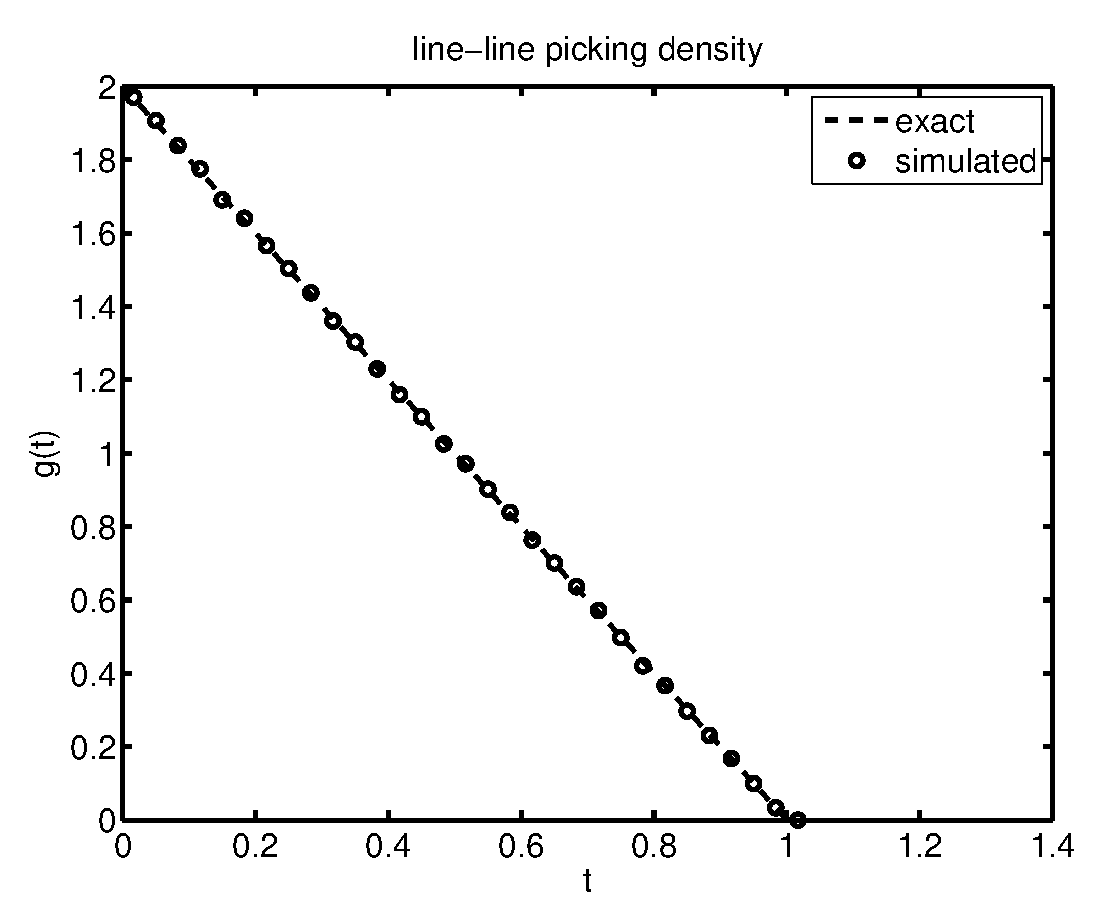
\includegraphics[width=0.32\columnwidth]{../Matlab/Plots/LinePicking_test_sim_line.eps}}
        \subfloat[square]{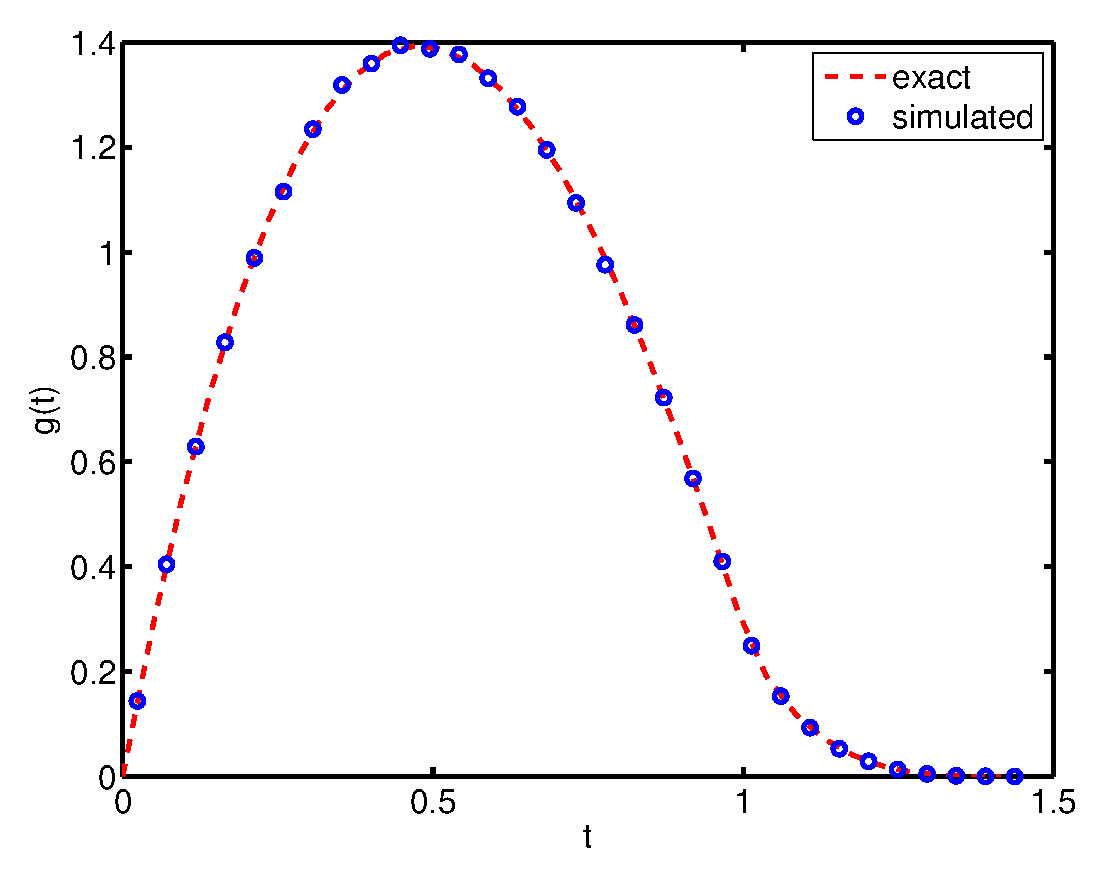
\includegraphics[width=0.32\columnwidth]{../Matlab/Plots/LinePicking_test_sim_square.eps}}
        \subfloat[cube]{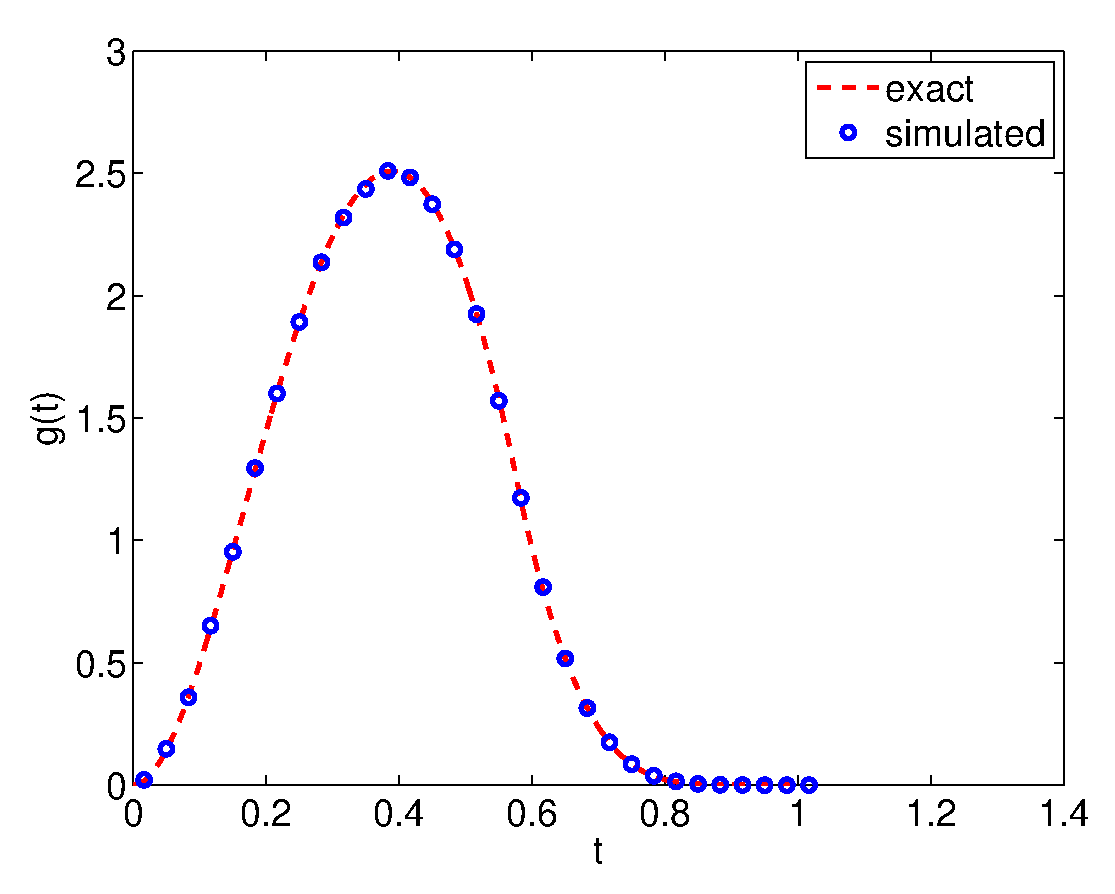
\includegraphics[width=0.32\columnwidth]{../Matlab/Plots/LinePicking_test_sim_cube.eps}}

        \subfloat[rectangle (1:2)]{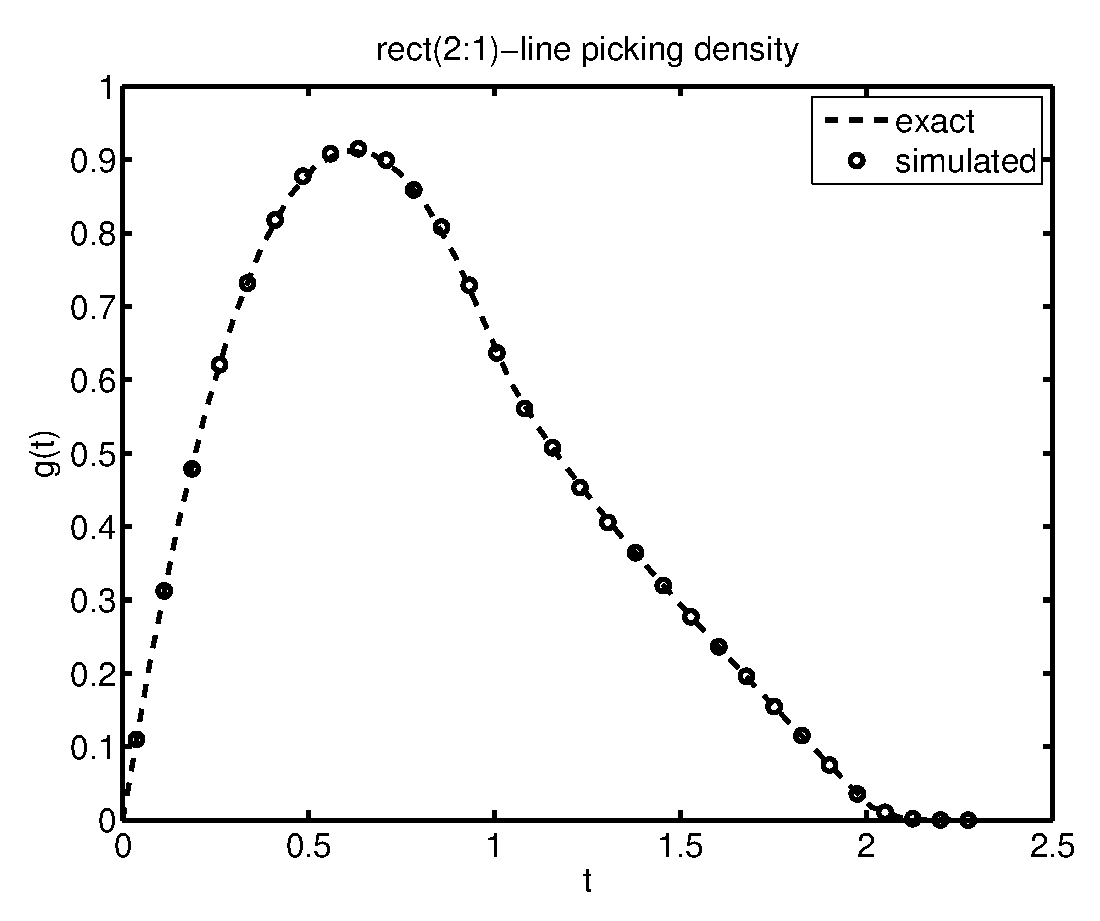
\includegraphics[width=0.32\columnwidth]{../Matlab/Plots/LinePicking_test_sim_rect.eps}}
        \subfloat[rectangle Manhattan (1:2)]{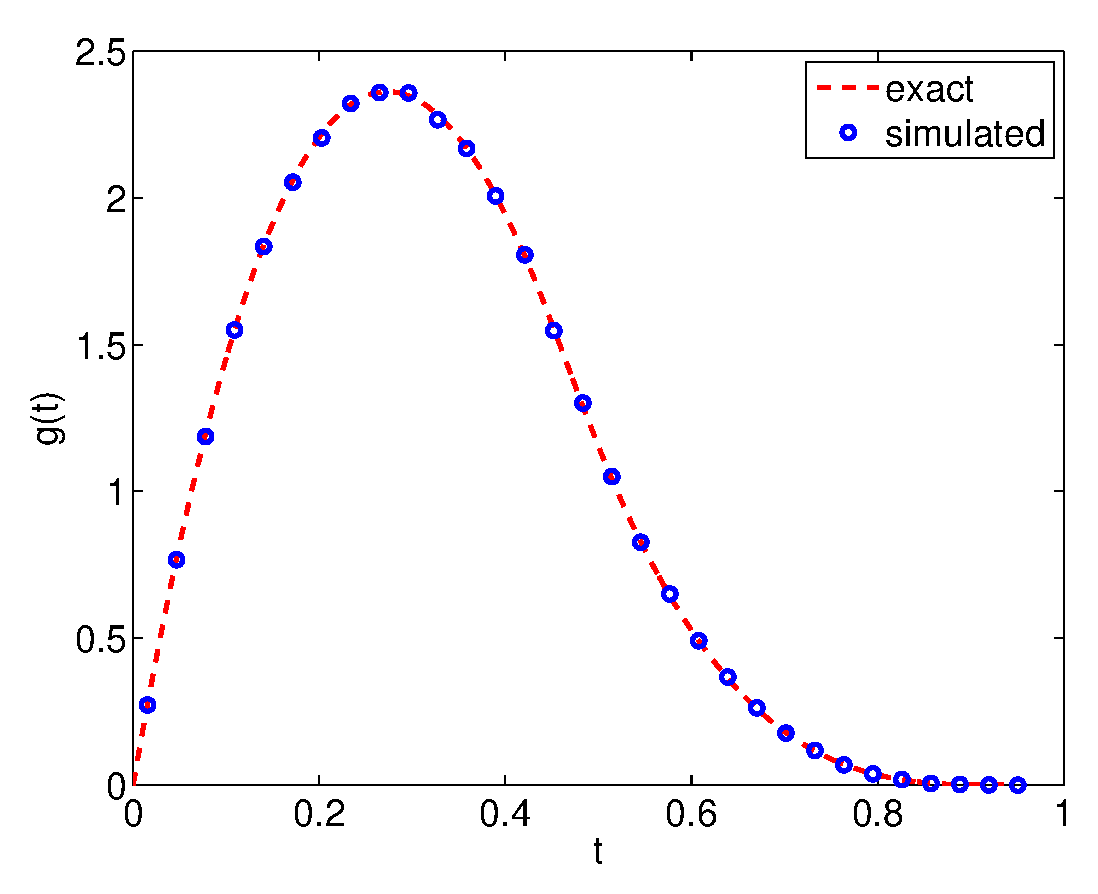
\includegraphics[width=0.32\columnwidth]{../Matlab/Plots/LinePicking_test_sim_rect_manhattan.eps}}
        \subfloat[rectangle max (1:2)]{\includegraphics[width=0.32\columnwidth]{../Matlab/Plots/LinePicking_test_sim_rectangle_max.eps}}

        \subfloat[disk (2-ball)]{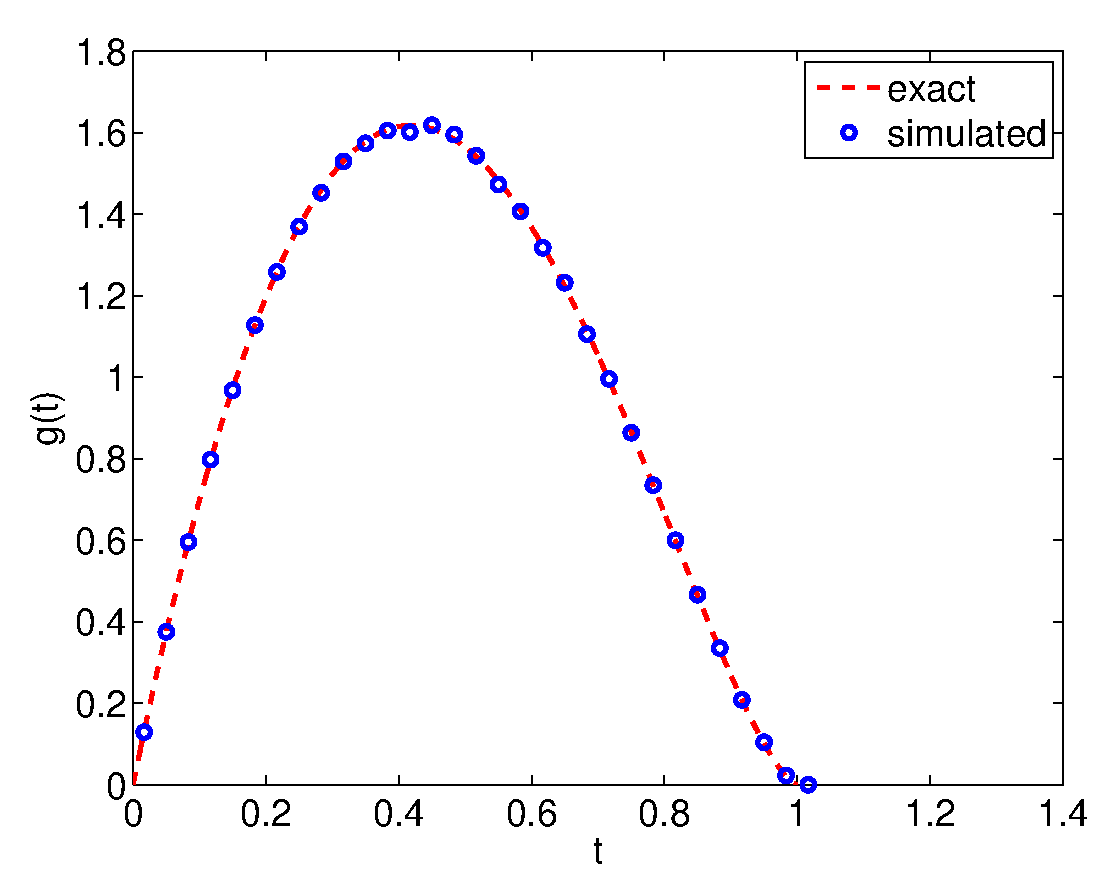
\includegraphics[width=0.32\columnwidth]{../Matlab/Plots/LinePicking_test_sim_disk.eps}}
        \subfloat[3-ball]{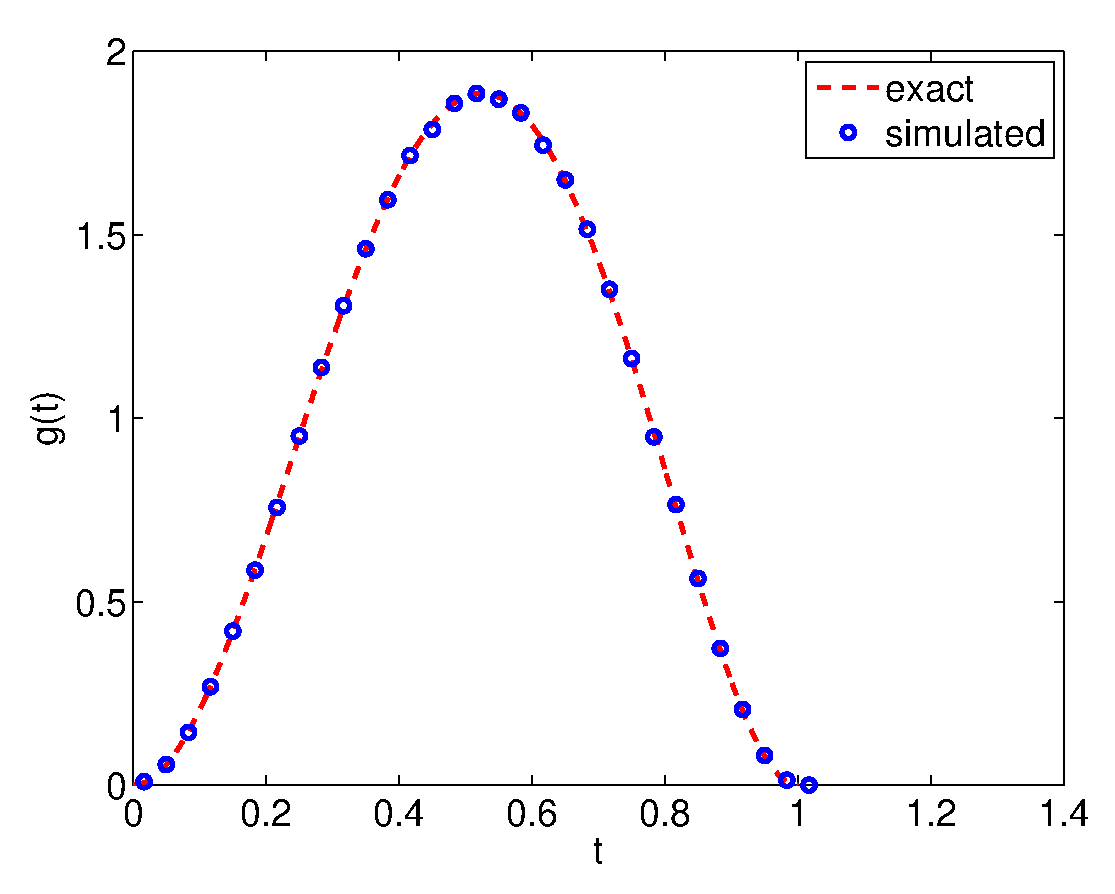
\includegraphics[width=0.32\columnwidth]{../Matlab/Plots/LinePicking_test_sim_3ball.eps}}
        \subfloat[4-ball]{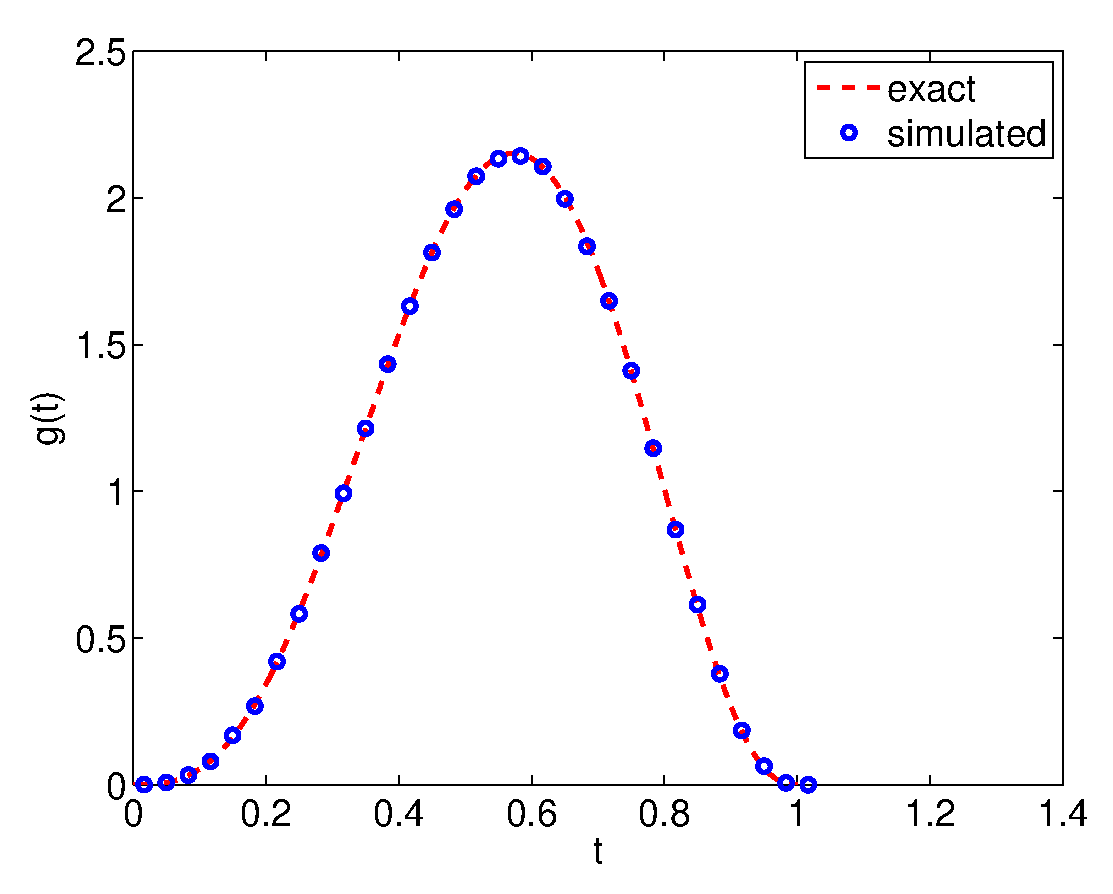
\includegraphics[width=0.32\columnwidth]{../Matlab/Plots/LinePicking_test_sim_4ball.eps}}

        \subfloat[circle (1-sphere)]{\includegraphics[width=0.32\columnwidth]{../Matlab/Plots/LinePicking_test_sim_circle.eps}}
        \subfloat[2-sphere]{\includegraphics[width=0.32\columnwidth]{../Matlab/Plots/LinePicking_test_sim_2-sphere.eps}}
        \subfloat[3-sphere]{\includegraphics[width=0.32\columnwidth]{../Matlab/Plots/LinePicking_test_sim_3sphere.eps}}

    \caption{\label{fig:sim_vs_exact}Comparisons of exactly calculated
      distributions and the distributions obtained by simulation. 
      1000000 simulated lines were used to draw the estimated PDF,
      which are binned into 30 equally spaced bins.}
  \end{center} 
\vspace{-4mm}
\end{figure}



\begin{figure}[tbp]
  \begin{center}
        \subfloat[circle geodesic]{\includegraphics[width=0.32\columnwidth]{../Matlab/Plots/LinePicking_test_sim_circle_geodesic.eps}}
        \subfloat[sphere geodesic]{\includegraphics[width=0.32\columnwidth]{../Matlab/Plots/LinePicking_test_sim_sphere_geodesic.eps}}
        \subfloat[3-sphere geodesic]{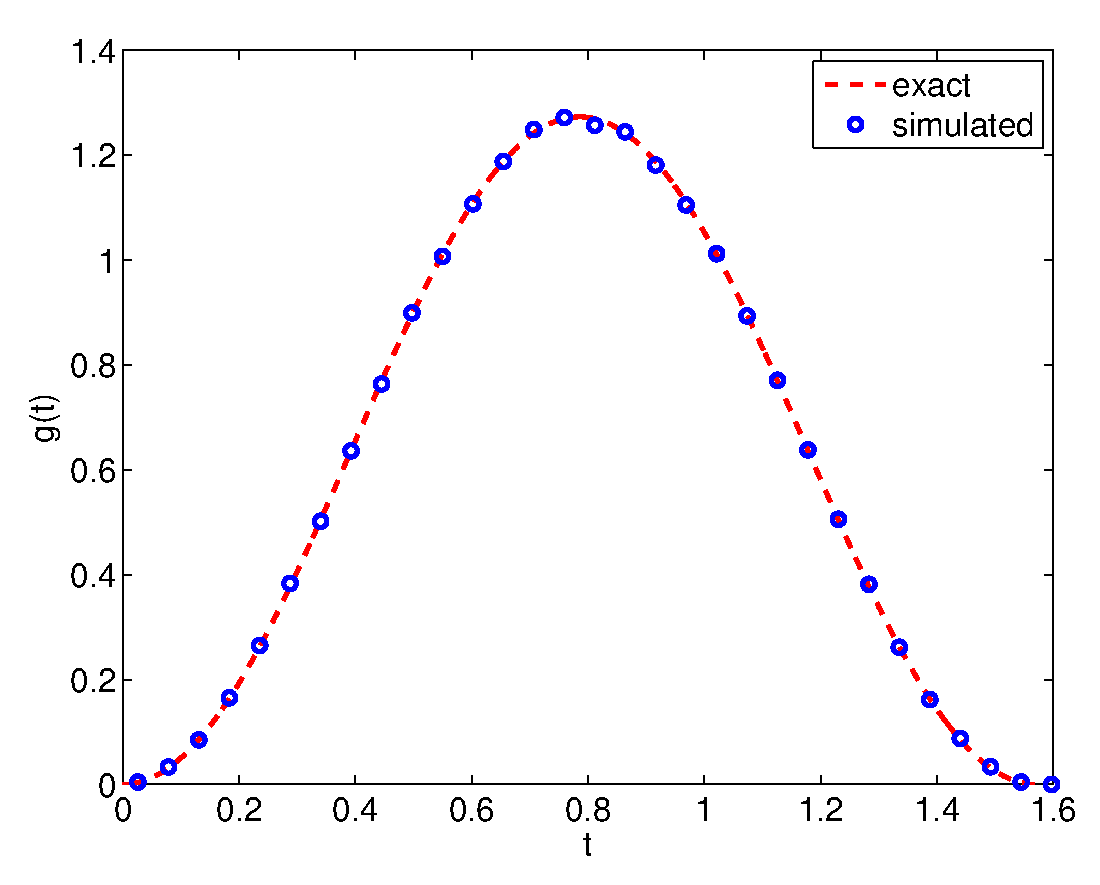
\includegraphics[width=0.32\columnwidth]{../Matlab/Plots/LinePicking_test_sim_3sphere_geodesic.eps}}

        \subfloat[prism geodesic]{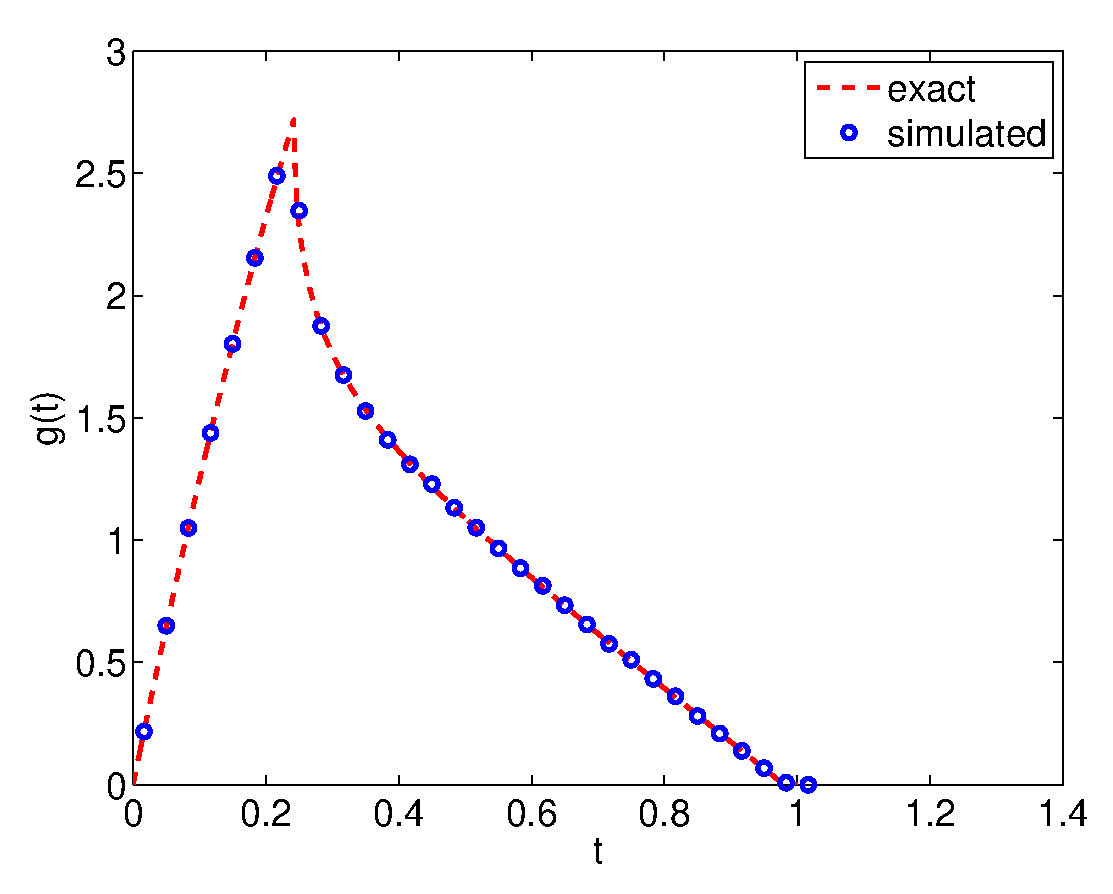
\includegraphics[width=0.32\columnwidth]{../Matlab/Plots/LinePicking_test_sim_prism_geodesic.eps}}
        \subfloat[cylindrical surface]{\includegraphics[width=0.32\columnwidth]{../Matlab/Plots/LinePicking_test_sim_cylindrical_surface.eps}}
        \subfloat[cylindrical surface geodesic]{\includegraphics[width=0.32\columnwidth]{../Matlab/Plots/LinePicking_test_sim_cylindrical_surface_geodesic.eps}}

        \subfloat[cylinder]{\includegraphics[width=0.32\columnwidth]{../Matlab/Plots/LinePicking_test_sim_cylinder.eps}}
        \subfloat[cube max]{\includegraphics[width=0.32\columnwidth]{../Matlab/Plots/LinePicking_test_sim_cube_max.eps}}
        \subfloat[4-cube max]{\includegraphics[width=0.32\columnwidth]{../Matlab/Plots/LinePicking_test_sim_4-cube_max.eps}}

    \caption{\label{fig:sim_vs_exact2}Comparisons of exactly calculated
      distributions and the distributions obtained by simulation. 
      1000000 simulated lines were used to draw the estimated PDF,
      which are binned into 30 equally spaced bins.}
  \end{center} 
\vspace{-4mm}
\end{figure}



\begin{table}[ht]
  \centering
  \begin{tabular}{r|rrrr}
                  problem &     mean & estimated mean & variance &  estimated var \\
     \hline 
                     line &   0.3333 &         0.3332 &   0.0556 &         0.0556 \\
                   square &   0.3687 &         0.3689 &   0.0307 &         0.0307 \\
                     cube &   0.3820 &         0.3820 &   0.0207 &         0.0207 \\
          rectangle (1:2) &   0.3599 &         0.3601 &   0.0371 &         0.0371 \\
rectangle Manhattan (1:2) &   0.3333 &         0.3335 &   0.0309 &         0.0308 \\
      rectangle max (1:2) &   0.3667 &         0.3711 &   0.0437 &         0.0437 \\
            disk (2-ball) &   0.4527 &         0.4529 &   0.0451 &         0.0451 \\
                   3-ball &   0.5143 &         0.5146 &   0.0355 &         0.0355 \\
                   4-ball &   0.5519 &         0.5521 &   0.0288 &         0.0288 \\
        circle (1-sphere) &   0.6366 &         0.6368 &   0.0947 &         0.0947 \\
                 2-sphere &   0.6667 &         0.6669 &   0.0556 &         0.0556 \\
                 3-sphere &   0.6791 &         0.6790 &   0.0389 &         0.0389 \\
          circle geodesic &   0.7854 &         0.7856 &   0.2056 &         0.2055 \\
          sphere geodesic &   0.7854 &         0.7857 &   0.1169 &         0.1170 \\
        3-sphere geodesic &   0.7854 &         0.7854 &   0.0806 &         0.0807 \\
           prism geodesic &   0.3645 &         0.3645 &   0.0436 &         0.0437 \\
      cylindrical surface &  -1.0000 &         0.4479 &  -1.0000 &         0.0327 \\
cylindrical surface geodesic &   0.4426 &         0.4426 &  -1.0000 &         0.0344 \\
                 cylinder &  -1.0000 &         0.3879 &  -1.0000 &         0.0328 \\
                 cube max &   0.5429 &         0.5428 &   0.0410 &         0.0410 \\
               4-cube max &   0.5937 &         0.5936 &   0.0349 &         0.0350 \\
  \end{tabular}
  \caption{Means and variances calculated exactly, and approximated by simulation.}
  \label{tab:mean_var_estimates}
\end{table}






\begin{table}[ht]
  \centering
  \begin{tabular}{r|r}
                  problem & PDF integral \\
     \hline 
                     line & 1.0000000000 \\
                   square & 1.0000000239 \\
                     cube & 1.0000000239 \\
          rectangle (1:2) & 0.9999999844 \\
rectangle Manhattan (1:2) & 0.9999999887 \\
      rectangle max (1:2) & 1.0000000000 \\
            disk (2-ball) & 1.0000000000 \\
                   3-ball & 1.0000000007 \\
                   4-ball & 1.0000000021 \\
        circle (1-sphere) & 1.0000000000 \\
                 2-sphere & 1.0000000000 \\
                 3-sphere & 1.0000000000 \\
          circle geodesic & 1.0000000000 \\
          sphere geodesic & 1.0000000000 \\
        3-sphere geodesic & 1.0000000000 \\
           prism geodesic & 0.9999999249 \\
      cylindrical surface & 0.9999977978 \\
cylindrical surface geodesic & 0.9999996398 \\
                 cylinder & 0.9999999620 \\
                 cube max & 1.0000000000 \\
               4-cube max & 1.0000000000 \\
  \end{tabular}
  \caption{Numerically integrated PDFs (integrated using Matlab's {\tt quadgk} function)}
  \label{tab:numerical_pdf_sum}
\end{table}


